\documentclass[1p]{elsarticle_modified}
%\bibliographystyle{elsarticle-num}

%\usepackage[colorlinks]{hyperref}
%\usepackage{abbrmath_seonhwa} %\Abb, \Ascr, \Acal ,\Abf, \Afrak
\usepackage{amsfonts}
\usepackage{amssymb}
\usepackage{amsmath}
\usepackage{amsthm}
\usepackage{scalefnt}
\usepackage{amsbsy}
\usepackage{kotex}
\usepackage{caption}
\usepackage{subfig}
\usepackage{color}
\usepackage{graphicx}
\usepackage{xcolor} %% white, black, red, green, blue, cyan, magenta, yellow
\usepackage{float}
\usepackage{setspace}
\usepackage{hyperref}

\usepackage{tikz}
\usetikzlibrary{arrows}

\usepackage{multirow}
\usepackage{array} % fixed length table
\usepackage{hhline}

%%%%%%%%%%%%%%%%%%%%%
\makeatletter
\renewcommand*\env@matrix[1][\arraystretch]{%
	\edef\arraystretch{#1}%
	\hskip -\arraycolsep
	\let\@ifnextchar\new@ifnextchar
	\array{*\c@MaxMatrixCols c}}
\makeatother %https://tex.stackexchange.com/questions/14071/how-can-i-increase-the-line-spacing-in-a-matrix
%%%%%%%%%%%%%%%

\usepackage[normalem]{ulem}

\newcommand{\msout}[1]{\ifmmode\text{\sout{\ensuremath{#1}}}\else\sout{#1}\fi}
%SOURCE: \msout is \stkout macro in https://tex.stackexchange.com/questions/20609/strikeout-in-math-mode

\newcommand{\cancel}[1]{
	\ifmmode
	{\color{red}\msout{#1}}
	\else
	{\color{red}\sout{#1}}
	\fi
}

\newcommand{\add}[1]{
	{\color{blue}\uwave{#1}}
}

\newcommand{\replace}[2]{
	\ifmmode
	{\color{red}\msout{#1}}{\color{blue}\uwave{#2}}
	\else
	{\color{red}\sout{#1}}{\color{blue}\uwave{#2}}
	\fi
}

\newcommand{\Sol}{\mathcal{S}} %segment
\newcommand{\D}{D} %diagram
\newcommand{\A}{\mathcal{A}} %arc


%%%%%%%%%%%%%%%%%%%%%%%%%%%%%5 test

\def\sl{\operatorname{\textup{SL}}(2,\Cbb)}
\def\psl{\operatorname{\textup{PSL}}(2,\Cbb)}
\def\quan{\mkern 1mu \triangleright \mkern 1mu}

\theoremstyle{definition}
\newtheorem{thm}{Theorem}[section]
\newtheorem{prop}[thm]{Proposition}
\newtheorem{lem}[thm]{Lemma}
\newtheorem{ques}[thm]{Question}
\newtheorem{cor}[thm]{Corollary}
\newtheorem{defn}[thm]{Definition}
\newtheorem{exam}[thm]{Example}
\newtheorem{rmk}[thm]{Remark}
\newtheorem{alg}[thm]{Algorithm}

\newcommand{\I}{\sqrt{-1}}
\begin{document}

%\begin{frontmatter}
%
%\title{Boundary parabolic representations of knots up to 8 crossings}
%
%%% Group authors per affiliation:
%\author{Yunhi Cho} 
%\address{Department of Mathematics, University of Seoul, Seoul, Korea}
%\ead{yhcho@uos.ac.kr}
%
%
%\author{Seonhwa Kim} %\fnref{s_kim}}
%\address{Center for Geometry and Physics, Institute for Basic Science, Pohang, 37673, Korea}
%\ead{ryeona17@ibs.re.kr}
%
%\author{Hyuk Kim}
%\address{Department of Mathematical Sciences, Seoul National University, Seoul 08826, Korea}
%\ead{hyukkim@snu.ac.kr}
%
%\author{Seokbeom Yoon}
%\address{Department of Mathematical Sciences, Seoul National University, Seoul, 08826,  Korea}
%\ead{sbyoon15@snu.ac.kr}
%
%\begin{abstract}
%We find all boundary parabolic representation of knots up to 8 crossings.
%
%\end{abstract}
%\begin{keyword}
%    \MSC[2010] 57M25 
%\end{keyword}
%
%\end{frontmatter}

%\linenumbers
%\tableofcontents
%
\newcommand\colored[1]{\textcolor{white}{\rule[-0.35ex]{0.8em}{1.4ex}}\kern-0.8em\color{red} #1}%
%\newcommand\colored[1]{\textcolor{white}{ #1}\kern-2.17ex	\textcolor{white}{ #1}\kern-1.81ex	\textcolor{white}{ #1}\kern-2.15ex\color{red}#1	}

{\Large $\underline{12n_{0502}~(K12n_{0502})}$}

\setlength{\tabcolsep}{10pt}
\renewcommand{\arraystretch}{1.6}
\vspace{1cm}\begin{tabular}{m{100pt}>{\centering\arraybackslash}m{274pt}}
\multirow{5}{120pt}{
	\centering
	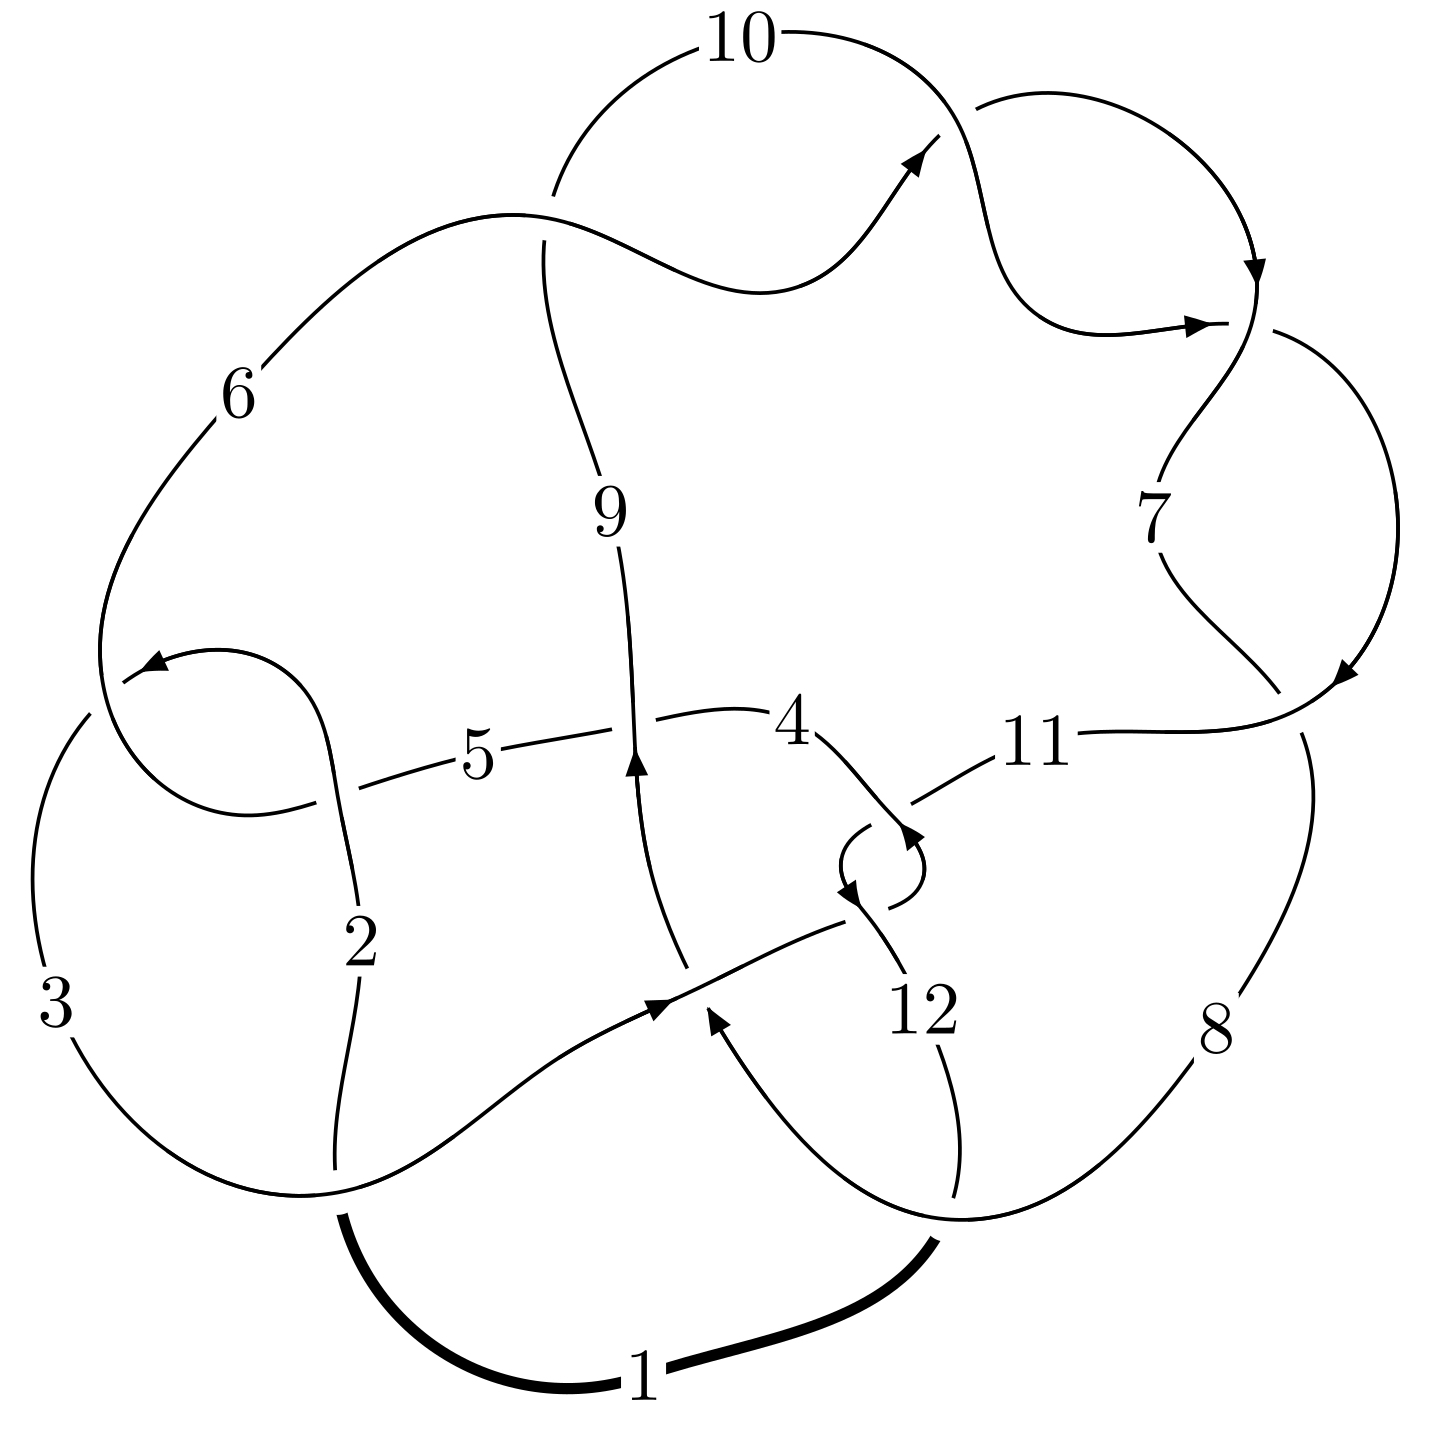
\includegraphics[width=112pt]{../../../GIT/diagram.site/Diagrams/png/2591_12n_0502.png}\\
\ \ \ A knot diagram\footnotemark}&
\allowdisplaybreaks
\textbf{Linearized knot diagam} \\
\cline{2-2}
 &
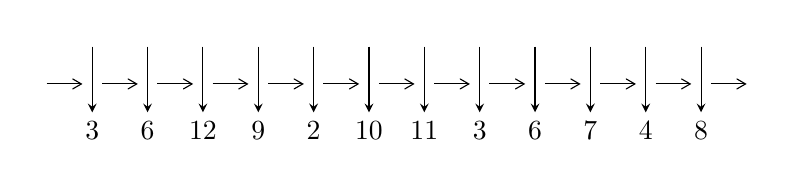
\begin{tikzpicture}[x=20pt, y=17pt]
	% nodes
	\node (C0) at (0, 0) {};
	\node (C1) at (1, 0) {};
	\node (C1U) at (1, +1) {};
	\node (C1D) at (1, -1) {3};

	\node (C2) at (2, 0) {};
	\node (C2U) at (2, +1) {};
	\node (C2D) at (2, -1) {6};

	\node (C3) at (3, 0) {};
	\node (C3U) at (3, +1) {};
	\node (C3D) at (3, -1) {12};

	\node (C4) at (4, 0) {};
	\node (C4U) at (4, +1) {};
	\node (C4D) at (4, -1) {9};

	\node (C5) at (5, 0) {};
	\node (C5U) at (5, +1) {};
	\node (C5D) at (5, -1) {2};

	\node (C6) at (6, 0) {};
	\node (C6U) at (6, +1) {};
	\node (C6D) at (6, -1) {10};

	\node (C7) at (7, 0) {};
	\node (C7U) at (7, +1) {};
	\node (C7D) at (7, -1) {11};

	\node (C8) at (8, 0) {};
	\node (C8U) at (8, +1) {};
	\node (C8D) at (8, -1) {3};

	\node (C9) at (9, 0) {};
	\node (C9U) at (9, +1) {};
	\node (C9D) at (9, -1) {6};

	\node (C10) at (10, 0) {};
	\node (C10U) at (10, +1) {};
	\node (C10D) at (10, -1) {7};

	\node (C11) at (11, 0) {};
	\node (C11U) at (11, +1) {};
	\node (C11D) at (11, -1) {4};

	\node (C12) at (12, 0) {};
	\node (C12U) at (12, +1) {};
	\node (C12D) at (12, -1) {8};
	\node (C13) at (13, 0) {};

	% arrows
	\draw[->,>={angle 60}]
	(C0) edge (C1) (C1) edge (C2) (C2) edge (C3) (C3) edge (C4) (C4) edge (C5) (C5) edge (C6) (C6) edge (C7) (C7) edge (C8) (C8) edge (C9) (C9) edge (C10) (C10) edge (C11) (C11) edge (C12) (C12) edge (C13) ;	\draw[->,>=stealth]
	(C1U) edge (C1D) (C2U) edge (C2D) (C3U) edge (C3D) (C4U) edge (C4D) (C5U) edge (C5D) (C6U) edge (C6D) (C7U) edge (C7D) (C8U) edge (C8D) (C9U) edge (C9D) (C10U) edge (C10D) (C11U) edge (C11D) (C12U) edge (C12D) ;
	\end{tikzpicture} \\
\hhline{~~} \\& 
\textbf{Solving Sequence} \\ \cline{2-2} 
 &
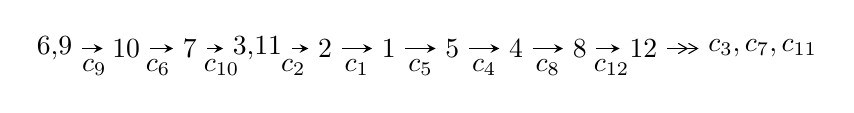
\begin{tikzpicture}[x=23pt, y=7pt]
	% node
	\node (A0) at (-1/8, 0) {6,9};
	\node (A1) at (1, 0) {10};
	\node (A2) at (2, 0) {7};
	\node (A3) at (49/16, 0) {3,11};
	\node (A4) at (33/8, 0) {2};
	\node (A5) at (41/8, 0) {1};
	\node (A6) at (49/8, 0) {5};
	\node (A7) at (57/8, 0) {4};
	\node (A8) at (65/8, 0) {8};
	\node (A9) at (73/8, 0) {12};
	\node (C1) at (1/2, -1) {$c_{9}$};
	\node (C2) at (3/2, -1) {$c_{6}$};
	\node (C3) at (5/2, -1) {$c_{10}$};
	\node (C4) at (29/8, -1) {$c_{2}$};
	\node (C5) at (37/8, -1) {$c_{1}$};
	\node (C6) at (45/8, -1) {$c_{5}$};
	\node (C7) at (53/8, -1) {$c_{4}$};
	\node (C8) at (61/8, -1) {$c_{8}$};
	\node (C9) at (69/8, -1) {$c_{12}$};
	\node (A10) at (11, 0) {$c_{3},c_{7},c_{11}$};

	% edge
	\draw[->,>=stealth]	
	(A0) edge (A1) (A1) edge (A2) (A2) edge (A3) (A3) edge (A4) (A4) edge (A5) (A5) edge (A6) (A6) edge (A7) (A7) edge (A8) (A8) edge (A9) ;
	\draw[->>,>={angle 60}]	
	(A9) edge (A10);
\end{tikzpicture} \\ 

\end{tabular} \\

\footnotetext{
The image of knot diagram is generated by the software ``\textbf{Draw programme}" developed by Andrew Bartholomew(\url{http://www.layer8.co.uk/maths/draw/index.htm\#Running-draw}), where we modified some parts for our purpose(\url{https://github.com/CATsTAILs/LinksPainter}).
}\phantom \\ \newline 
\centering \textbf{Ideals for irreducible components\footnotemark of $X_{\text{par}}$} 
 
\begin{align*}
I^u_{1}&=\langle 
- u^9-2 u^8+5 u^7+11 u^6-2 u^5-14 u^4-15 u^3-6 u^2+2 b- u-1,\\
\phantom{I^u_{1}}&\phantom{= \langle  }- u^9-2 u^8+7 u^7+15 u^6-14 u^5-38 u^4+u^3+32 u^2+4 a+11 u-3,\\
\phantom{I^u_{1}}&\phantom{= \langle  }u^{10}+4 u^9-2 u^8-24 u^7-16 u^6+35 u^5+44 u^4+11 u^3- u^2+3 u+1\rangle \\
I^u_{2}&=\langle 
b,\;a^3+a^2 u- a^2-2 u+3,\;u^2- u-1\rangle \\
\\
\end{align*}
\raggedright * 2 irreducible components of $\dim_{\mathbb{C}}=0$, with total 16 representations.\\
\footnotetext{All coefficients of polynomials are rational numbers. But the coefficients are sometimes approximated in decimal forms when there is not enough margin.}
\newpage
\renewcommand{\arraystretch}{1}
\centering \section*{I. $I^u_{1}= \langle - u^9-2 u^8+\cdots+2 b-1,\;- u^9-2 u^8+\cdots+4 a-3,\;u^{10}+4 u^9+\cdots+3 u+1 \rangle$}
\flushleft \textbf{(i) Arc colorings}\\
\begin{tabular}{m{7pt} m{180pt} m{7pt} m{180pt} }
\flushright $a_{6}=$&$\begin{pmatrix}0\\u\end{pmatrix}$ \\
\flushright $a_{9}=$&$\begin{pmatrix}1\\0\end{pmatrix}$ \\
\flushright $a_{10}=$&$\begin{pmatrix}1\\u^2\end{pmatrix}$ \\
\flushright $a_{7}=$&$\begin{pmatrix}- u\\- u^3+u\end{pmatrix}$ \\
\flushright $a_{3}=$&$\begin{pmatrix}\frac{1}{4} u^9+\frac{1}{2} u^8+\cdots-\frac{11}{4} u+\frac{3}{4}\\\frac{1}{2} u^9+u^8+\cdots+\frac{1}{2} u+\frac{1}{2}\end{pmatrix}$ \\
\flushright $a_{11}=$&$\begin{pmatrix}- u^2+1\\- u^4+2 u^2\end{pmatrix}$ \\
\flushright $a_{2}=$&$\begin{pmatrix}\frac{1}{4} u^9+\frac{1}{2} u^8+\cdots-\frac{11}{4} u+\frac{3}{4}\\-\frac{1}{4} u^9-\frac{1}{4} u^8+\cdots+\frac{7}{2} u^2-\frac{3}{4} u\end{pmatrix}$ \\
\flushright $a_{1}=$&$\begin{pmatrix}-\frac{7}{4} u^9-\frac{13}{4} u^8+\cdots-\frac{7}{4} u+\frac{1}{2}\\-\frac{25}{4} u^9-\frac{45}{4} u^8+\cdots-\frac{35}{4} u-3\end{pmatrix}$ \\
\flushright $a_{5}=$&$\begin{pmatrix}-\frac{1}{4} u^8-\frac{3}{4} u^7+\cdots-3 u-\frac{3}{4}\\-\frac{1}{4} u^9-\frac{1}{2} u^8+\cdots+\frac{5}{4} u-\frac{1}{4}\end{pmatrix}$ \\
\flushright $a_{4}=$&$\begin{pmatrix}-\frac{1}{4} u^9-\frac{3}{4} u^8+\cdots-\frac{7}{4} u-1\\-\frac{1}{4} u^9-\frac{1}{2} u^8+\cdots+\frac{5}{4} u-\frac{1}{4}\end{pmatrix}$ \\
\flushright $a_{8}=$&$\begin{pmatrix}u^3-2 u\\u^5-3 u^3+u\end{pmatrix}$ \\
\flushright $a_{12}=$&$\begin{pmatrix}-\frac{1}{2} u^8- u^7+\cdots+\frac{1}{2} u+\frac{3}{2}\\\frac{3}{4} u^9+\frac{7}{4} u^8+\cdots+\frac{5}{2} u^2-\frac{3}{4} u\end{pmatrix}$\\&\end{tabular}
\flushleft \textbf{(ii) Obstruction class $= -1$}\\~\\
\flushleft \textbf{(iii) Cusp Shapes $= - u^9-5 u^8+\frac{61}{2} u^6+29 u^5-\frac{91}{2} u^4-68 u^3-15 u^2+\frac{15}{2} u-\frac{29}{2}$}\\~\\
\newpage\renewcommand{\arraystretch}{1}
\flushleft \textbf{(iv) u-Polynomials at the component}\newline \\
\begin{tabular}{m{50pt}|m{274pt}}
Crossings & \hspace{64pt}u-Polynomials at each crossing \\
\hline $$\begin{aligned}c_{1}\end{aligned}$$&$\begin{aligned}
&u^{10}+29 u^9+\cdots-19 u+4
\end{aligned}$\\
\hline $$\begin{aligned}c_{2},c_{5}\end{aligned}$$&$\begin{aligned}
&u^{10}+3 u^9-10 u^8-34 u^7-17 u^6+7 u^5+59 u^4-55 u^3-11 u^2-5 u-2
\end{aligned}$\\
\hline $$\begin{aligned}c_{3},c_{11}\end{aligned}$$&$\begin{aligned}
&u^{10}-3 u^9+8 u^8-13 u^7+18 u^6-20 u^5+16 u^4-11 u^3+3 u^2-2 u-1
\end{aligned}$\\
\hline $$\begin{aligned}c_{4}\end{aligned}$$&$\begin{aligned}
&u^{10}-25 u^9+\cdots-1689 u-389
\end{aligned}$\\
\hline $$\begin{aligned}c_{6},c_{7},c_{9}\\c_{10}\end{aligned}$$&$\begin{aligned}
&u^{10}+4 u^9-2 u^8-24 u^7-16 u^6+35 u^5+44 u^4+11 u^3- u^2+3 u+1
\end{aligned}$\\
\hline $$\begin{aligned}c_{8}\end{aligned}$$&$\begin{aligned}
&u^{10}+u^9+\cdots-160 u-64
\end{aligned}$\\
\hline $$\begin{aligned}c_{12}\end{aligned}$$&$\begin{aligned}
&u^{10}-2 u^9-11 u^8+16 u^7+23 u^6+10 u^5- u^4+5 u^3+6 u^2+4 u+1
\end{aligned}$\\
\hline
\end{tabular}\\~\\
\newpage\renewcommand{\arraystretch}{1}
\flushleft \textbf{(v) Riley Polynomials at the component}\newline \\
\begin{tabular}{m{50pt}|m{274pt}}
Crossings & \hspace{64pt}Riley Polynomials at each crossing \\
\hline $$\begin{aligned}c_{1}\end{aligned}$$&$\begin{aligned}
&y^{10}-301 y^9+\cdots-5681 y+16
\end{aligned}$\\
\hline $$\begin{aligned}c_{2},c_{5}\end{aligned}$$&$\begin{aligned}
&y^{10}-29 y^9+\cdots+19 y+4
\end{aligned}$\\
\hline $$\begin{aligned}c_{3},c_{11}\end{aligned}$$&$\begin{aligned}
&y^{10}+7 y^9+22 y^8+31 y^7-76 y^5-144 y^4-141 y^3-67 y^2-10 y+1
\end{aligned}$\\
\hline $$\begin{aligned}c_{4}\end{aligned}$$&$\begin{aligned}
&y^{10}-169 y^9+\cdots-1357405 y+151321
\end{aligned}$\\
\hline $$\begin{aligned}c_{6},c_{7},c_{9}\\c_{10}\end{aligned}$$&$\begin{aligned}
&y^{10}-20 y^9+\cdots-11 y+1
\end{aligned}$\\
\hline $$\begin{aligned}c_{8}\end{aligned}$$&$\begin{aligned}
&y^{10}-35 y^9+\cdots-5120 y+4096
\end{aligned}$\\
\hline $$\begin{aligned}c_{12}\end{aligned}$$&$\begin{aligned}
&y^{10}-26 y^9+\cdots-4 y+1
\end{aligned}$\\
\hline
\end{tabular}\\~\\
\newpage\flushleft \textbf{(vi) Complex Volumes and Cusp Shapes}
$$\begin{array}{c|c|c}  
\text{Solutions to }I^u_{1}& \I (\text{vol} + \sqrt{-1}CS) & \text{Cusp shape}\\
 \hline 
\begin{aligned}
u &= -0.770282 + 0.350441 I \\
a &= -0.175699 + 0.338848 I \\
b &= \phantom{-}0.722401 + 0.709455 I\end{aligned}
 & -0.295773 + 0.495817 I & -13.91306 - 1.36095 I \\ \hline\begin{aligned}
u &= -0.770282 - 0.350441 I \\
a &= -0.175699 - 0.338848 I \\
b &= \phantom{-}0.722401 - 0.709455 I\end{aligned}
 & -0.295773 - 0.495817 I & -13.91306 + 1.36095 I \\ \hline\begin{aligned}
u &= \phantom{-}0.238689 + 0.328179 I \\
a &= \phantom{-}0.29003 - 2.34120 I \\
b &= -0.187083 + 0.681344 I\end{aligned}
 & \phantom{-}2.64731 + 2.28565 I & -6.52151 - 0.97940 I \\ \hline\begin{aligned}
u &= \phantom{-}0.238689 - 0.328179 I \\
a &= \phantom{-}0.29003 + 2.34120 I \\
b &= -0.187083 - 0.681344 I\end{aligned}
 & \phantom{-}2.64731 - 2.28565 I & -6.52151 + 0.97940 I \\ \hline\begin{aligned}
u &= -0.293390\phantom{ +0.000000I} \\
a &= \phantom{-}0.935254\phantom{ +0.000000I} \\
b &= \phantom{-}0.468829\phantom{ +0.000000I}\end{aligned}
 & -0.595897\phantom{ +0.000000I} & -16.6550\phantom{ +0.000000I} \\ \hline\begin{aligned}
u &= \phantom{-}1.78423 + 0.22622 I \\
a &= -0.335255 + 0.782997 I \\
b &= -1.44386 + 1.68806 I\end{aligned}
 & -9.27245 - 2.54510 I & -15.8897 + 2.0711 I \\ \hline\begin{aligned}
u &= \phantom{-}1.78423 - 0.22622 I \\
a &= -0.335255 - 0.782997 I \\
b &= -1.44386 - 1.68806 I\end{aligned}
 & -9.27245 + 2.54510 I & -15.8897 - 2.0711 I \\ \hline\begin{aligned}
u &= -2.03029 + 0.17685 I \\
a &= \phantom{-}1.52970 + 0.03504 I \\
b &= \phantom{-}3.31663 - 1.27082 I\end{aligned}
 & \phantom{-}15.1518 + 6.6636 I & -15.1690 - 2.5369 I \\ \hline\begin{aligned}
u &= -2.03029 - 0.17685 I \\
a &= \phantom{-}1.52970 - 0.03504 I \\
b &= \phantom{-}3.31663 + 1.27082 I\end{aligned}
 & \phantom{-}15.1518 - 6.6636 I & -15.1690 + 2.5369 I \\ \hline\begin{aligned}
u &= -2.15130\phantom{ +0.000000I} \\
a &= -1.55281\phantom{ +0.000000I} \\
b &= -4.28499\phantom{ +0.000000I}\end{aligned}
 & \phantom{-}10.4531\phantom{ +0.000000I} & -17.3580\phantom{ +0.000000I}\\
 \hline 
 \end{array}$$\newpage\newpage\renewcommand{\arraystretch}{1}
\centering \section*{II. $I^u_{2}= \langle b,\;a^3+a^2 u- a^2-2 u+3,\;u^2- u-1 \rangle$}
\flushleft \textbf{(i) Arc colorings}\\
\begin{tabular}{m{7pt} m{180pt} m{7pt} m{180pt} }
\flushright $a_{6}=$&$\begin{pmatrix}0\\u\end{pmatrix}$ \\
\flushright $a_{9}=$&$\begin{pmatrix}1\\0\end{pmatrix}$ \\
\flushright $a_{10}=$&$\begin{pmatrix}1\\u+1\end{pmatrix}$ \\
\flushright $a_{7}=$&$\begin{pmatrix}- u\\- u-1\end{pmatrix}$ \\
\flushright $a_{3}=$&$\begin{pmatrix}a\\0\end{pmatrix}$ \\
\flushright $a_{11}=$&$\begin{pmatrix}- u\\- u\end{pmatrix}$ \\
\flushright $a_{2}=$&$\begin{pmatrix}a\\- a u- a\end{pmatrix}$ \\
\flushright $a_{1}=$&$\begin{pmatrix}a^2 u+a- u+1\\- a u- a\end{pmatrix}$ \\
\flushright $a_{5}=$&$\begin{pmatrix}a^2 u\\-2 a^2 u- a^2+u\end{pmatrix}$ \\
\flushright $a_{4}=$&$\begin{pmatrix}- a^2 u- a^2+u\\-2 a^2 u- a^2+u\end{pmatrix}$ \\
\flushright $a_{8}=$&$\begin{pmatrix}1\\0\end{pmatrix}$ \\
\flushright $a_{12}=$&$\begin{pmatrix}a^2 u- a u- u+1\\- a u- a\end{pmatrix}$\\&\end{tabular}
\flushleft \textbf{(ii) Obstruction class $= 1$}\\~\\
\flushleft \textbf{(iii) Cusp Shapes $= a^2-2 a u+a+u-17$}\\~\\
\newpage\renewcommand{\arraystretch}{1}
\flushleft \textbf{(iv) u-Polynomials at the component}\newline \\
\begin{tabular}{m{50pt}|m{274pt}}
Crossings & \hspace{64pt}u-Polynomials at each crossing \\
\hline $$\begin{aligned}c_{1},c_{11}\end{aligned}$$&$\begin{aligned}
&(u^3- u^2+2 u-1)^2
\end{aligned}$\\
\hline $$\begin{aligned}c_{2}\end{aligned}$$&$\begin{aligned}
&(u^3+u^2-1)^2
\end{aligned}$\\
\hline $$\begin{aligned}c_{3}\end{aligned}$$&$\begin{aligned}
&(u^3+u^2+2 u+1)^2
\end{aligned}$\\
\hline $$\begin{aligned}c_{4}\end{aligned}$$&$\begin{aligned}
&u^6+2 u^5+5 u^4-2 u^3+3 u^2+3 u-1
\end{aligned}$\\
\hline $$\begin{aligned}c_{5}\end{aligned}$$&$\begin{aligned}
&(u^3- u^2+1)^2
\end{aligned}$\\
\hline $$\begin{aligned}c_{6},c_{7}\end{aligned}$$&$\begin{aligned}
&(u^2+u-1)^3
\end{aligned}$\\
\hline $$\begin{aligned}c_{8}\end{aligned}$$&$\begin{aligned}
&u^6
\end{aligned}$\\
\hline $$\begin{aligned}c_{9},c_{10}\end{aligned}$$&$\begin{aligned}
&(u^2- u-1)^3
\end{aligned}$\\
\hline $$\begin{aligned}c_{12}\end{aligned}$$&$\begin{aligned}
&u^6+u^5- u^4-4 u^3+3 u^2-1
\end{aligned}$\\
\hline
\end{tabular}\\~\\
\newpage\renewcommand{\arraystretch}{1}
\flushleft \textbf{(v) Riley Polynomials at the component}\newline \\
\begin{tabular}{m{50pt}|m{274pt}}
Crossings & \hspace{64pt}Riley Polynomials at each crossing \\
\hline $$\begin{aligned}c_{1},c_{3},c_{11}\end{aligned}$$&$\begin{aligned}
&(y^3+3 y^2+2 y-1)^2
\end{aligned}$\\
\hline $$\begin{aligned}c_{2},c_{5}\end{aligned}$$&$\begin{aligned}
&(y^3- y^2+2 y-1)^2
\end{aligned}$\\
\hline $$\begin{aligned}c_{4}\end{aligned}$$&$\begin{aligned}
&y^6+6 y^5+39 y^4+12 y^3+11 y^2-15 y+1
\end{aligned}$\\
\hline $$\begin{aligned}c_{6},c_{7},c_{9}\\c_{10}\end{aligned}$$&$\begin{aligned}
&(y^2-3 y+1)^3
\end{aligned}$\\
\hline $$\begin{aligned}c_{8}\end{aligned}$$&$\begin{aligned}
&y^6
\end{aligned}$\\
\hline $$\begin{aligned}c_{12}\end{aligned}$$&$\begin{aligned}
&y^6-3 y^5+15 y^4-24 y^3+11 y^2-6 y+1
\end{aligned}$\\
\hline
\end{tabular}\\~\\
\newpage\flushleft \textbf{(vi) Complex Volumes and Cusp Shapes}
$$\begin{array}{c|c|c}  
\text{Solutions to }I^u_{2}& \I (\text{vol} + \sqrt{-1}CS) & \text{Cusp shape}\\
 \hline 
\begin{aligned}
u &= -0.618034\phantom{ +0.000000I} \\
a &= -1.22142\phantom{ +0.000000I} \\
b &= \phantom{-0.000000 } 0\end{aligned}
 & -2.10041\phantom{ +0.000000I} & -18.8570\phantom{ +0.000000I} \\ \hline\begin{aligned}
u &= -0.618034\phantom{ +0.000000I} \\
a &= \phantom{-}1.41973 + 1.20521 I \\
b &= \phantom{-0.000000 } 0\end{aligned}
 & \phantom{-}2.03717 - 2.82812 I & -13.8803 + 6.1171 I \\ \hline\begin{aligned}
u &= -0.618034\phantom{ +0.000000I} \\
a &= \phantom{-}1.41973 - 1.20521 I \\
b &= \phantom{-0.000000 } 0\end{aligned}
 & \phantom{-}2.03717 + 2.82812 I & -13.8803 - 6.1171 I \\ \hline\begin{aligned}
u &= \phantom{-}1.61803\phantom{ +0.000000I} \\
a &= -0.542287 + 0.460350 I \\
b &= \phantom{-0.000000 } 0\end{aligned}
 & -5.85852 + 2.82812 I & -14.0872 - 1.5287 I \\ \hline\begin{aligned}
u &= \phantom{-}1.61803\phantom{ +0.000000I} \\
a &= -0.542287 - 0.460350 I \\
b &= \phantom{-0.000000 } 0\end{aligned}
 & -5.85852 - 2.82812 I & -14.0872 + 1.5287 I \\ \hline\begin{aligned}
u &= \phantom{-}1.61803\phantom{ +0.000000I} \\
a &= \phantom{-}0.466540\phantom{ +0.000000I} \\
b &= \phantom{-0.000000 } 0\end{aligned}
 & -9.99610\phantom{ +0.000000I} & -16.2080\phantom{ +0.000000I}\\
 \hline 
 \end{array}$$\newpage
\newpage\renewcommand{\arraystretch}{1}
\centering \section*{ III. u-Polynomials}
\begin{tabular}{m{50pt}|m{274pt}}
Crossings & \hspace{64pt}u-Polynomials at each crossing \\
\hline $$\begin{aligned}c_{1}\end{aligned}$$&$\begin{aligned}
&((u^3- u^2+2 u-1)^2)(u^{10}+29 u^9+\cdots-19 u+4)
\end{aligned}$\\
\hline $$\begin{aligned}c_{2}\end{aligned}$$&$\begin{aligned}
&(u^3+u^2-1)^2\\
&\cdot(u^{10}+3 u^9-10 u^8-34 u^7-17 u^6+7 u^5+59 u^4-55 u^3-11 u^2-5 u-2)
\end{aligned}$\\
\hline $$\begin{aligned}c_{3}\end{aligned}$$&$\begin{aligned}
&(u^3+u^2+2 u+1)^2\\
&\cdot(u^{10}-3 u^9+8 u^8-13 u^7+18 u^6-20 u^5+16 u^4-11 u^3+3 u^2-2 u-1)
\end{aligned}$\\
\hline $$\begin{aligned}c_{4}\end{aligned}$$&$\begin{aligned}
&(u^6+2 u^5+\cdots+3 u-1)(u^{10}-25 u^9+\cdots-1689 u-389)
\end{aligned}$\\
\hline $$\begin{aligned}c_{5}\end{aligned}$$&$\begin{aligned}
&(u^3- u^2+1)^2\\
&\cdot(u^{10}+3 u^9-10 u^8-34 u^7-17 u^6+7 u^5+59 u^4-55 u^3-11 u^2-5 u-2)
\end{aligned}$\\
\hline $$\begin{aligned}c_{6},c_{7}\end{aligned}$$&$\begin{aligned}
&(u^2+u-1)^3\\
&\cdot(u^{10}+4 u^9-2 u^8-24 u^7-16 u^6+35 u^5+44 u^4+11 u^3- u^2+3 u+1)
\end{aligned}$\\
\hline $$\begin{aligned}c_{8}\end{aligned}$$&$\begin{aligned}
&u^6(u^{10}+u^9+\cdots-160 u-64)
\end{aligned}$\\
\hline $$\begin{aligned}c_{9},c_{10}\end{aligned}$$&$\begin{aligned}
&(u^2- u-1)^3\\
&\cdot(u^{10}+4 u^9-2 u^8-24 u^7-16 u^6+35 u^5+44 u^4+11 u^3- u^2+3 u+1)
\end{aligned}$\\
\hline $$\begin{aligned}c_{11}\end{aligned}$$&$\begin{aligned}
&(u^3- u^2+2 u-1)^2\\
&\cdot(u^{10}-3 u^9+8 u^8-13 u^7+18 u^6-20 u^5+16 u^4-11 u^3+3 u^2-2 u-1)
\end{aligned}$\\
\hline $$\begin{aligned}c_{12}\end{aligned}$$&$\begin{aligned}
&(u^6+u^5- u^4-4 u^3+3 u^2-1)\\
&\cdot(u^{10}-2 u^9-11 u^8+16 u^7+23 u^6+10 u^5- u^4+5 u^3+6 u^2+4 u+1)
\end{aligned}$\\
\hline
\end{tabular}\newpage\renewcommand{\arraystretch}{1}
\centering \section*{ IV. Riley Polynomials}
\begin{tabular}{m{50pt}|m{274pt}}
Crossings & \hspace{64pt}Riley Polynomials at each crossing \\
\hline $$\begin{aligned}c_{1}\end{aligned}$$&$\begin{aligned}
&((y^3+3 y^2+2 y-1)^2)(y^{10}-301 y^9+\cdots-5681 y+16)
\end{aligned}$\\
\hline $$\begin{aligned}c_{2},c_{5}\end{aligned}$$&$\begin{aligned}
&((y^3- y^2+2 y-1)^2)(y^{10}-29 y^9+\cdots+19 y+4)
\end{aligned}$\\
\hline $$\begin{aligned}c_{3},c_{11}\end{aligned}$$&$\begin{aligned}
&(y^3+3 y^2+2 y-1)^2\\
&\cdot(y^{10}+7 y^9+22 y^8+31 y^7-76 y^5-144 y^4-141 y^3-67 y^2-10 y+1)
\end{aligned}$\\
\hline $$\begin{aligned}c_{4}\end{aligned}$$&$\begin{aligned}
&(y^6+6 y^5+39 y^4+12 y^3+11 y^2-15 y+1)\\
&\cdot(y^{10}-169 y^9+\cdots-1357405 y+151321)
\end{aligned}$\\
\hline $$\begin{aligned}c_{6},c_{7},c_{9}\\c_{10}\end{aligned}$$&$\begin{aligned}
&((y^2-3 y+1)^3)(y^{10}-20 y^9+\cdots-11 y+1)
\end{aligned}$\\
\hline $$\begin{aligned}c_{8}\end{aligned}$$&$\begin{aligned}
&y^6(y^{10}-35 y^9+\cdots-5120 y+4096)
\end{aligned}$\\
\hline $$\begin{aligned}c_{12}\end{aligned}$$&$\begin{aligned}
&(y^6-3 y^5+\cdots-6 y+1)(y^{10}-26 y^9+\cdots-4 y+1)
\end{aligned}$\\
\hline
\end{tabular}
\vskip 2pc
\end{document}